% 
% Annual Cognitive Science Conference
% Sample LaTeX Paper -- Proceedings Format
% 

% Original : Ashwin Ram (ashwin@cc.gatech.edu)       04/01/1994
% Modified : Johanna Moore (jmoore@cs.pitt.edu)      03/17/1995
% Modified : David Noelle (noelle@ucsd.edu)          03/15/1996
% Modified : Pat Langley (langley@cs.stanford.edu)   01/26/1997
% Latex2e corrections by Ramin Charles Nakisa        01/28/1997 
% Modified : Tina Eliassi-Rad (eliassi@cs.wisc.edu)  01/31/1998
% Modified : Trisha Yannuzzi (trisha@ircs.upenn.edu) 12/28/1999 (in process)
% Modified : Mary Ellen Foster (M.E.Foster@ed.ac.uk) 12/11/2000
% Modified : Ken Forbus                              01/23/2004
% Modified : Eli M. Silk (esilk@pitt.edu)            05/24/2005
% Modified : Niels Taatgen (taatgen@cmu.edu)         10/24/2006
% Modified : David Noelle (dnoelle@ucmerced.edu)     11/19/2014

%% Change "letterpaper" in the following line to "a4paper" if you must.

\documentclass[10pt,letterpaper]{article}
\newcommand\tab[1][0.5cm]{\hspace*{#1}}
\usepackage{cogsci}
\usepackage{pslatex}
\usepackage{hyperref}
\usepackage{apacite}
\usepackage{graphicx}
\usepackage{amsmath}
\usepackage{amssymb}
\usepackage[usenames, dvipsnames]{color}

 \newcommand{\denote}[1]{\mbox{ $[\![ #1 ]\!]$}}

\definecolor{Green}{RGB}{10,200,100}
\newcommand{\ndg}[1]{\textcolor{Green}{[ndg: #1]}}

\title{[Cute title]: The Pragmatics of Spatial Language}
 
%\author{{\large \bf Morton Ann Gernsbacher (MAG@Macc.Wisc.Edu)} \\
%  Department of Psychology, 1202 W. Johnson Street \\
%  Madison, WI 53706 USA
%  \AND {\large \bf Sharon J.~Derry (SDJ@Macc.Wisc.Edu)} \\
%  Department of Educational Psychology, 1025 W. Johnson Street \\
%  Madison, WI 53706 USA}

\author{
{\large \bf Author 1 (email@place.edu)} \\
  Department of Psychology, University of Gondor\\
  \And{\large \bf Author 2 (email@place.edu)} \\
  Department of Cognitive Science, University of Mordor \\
  \\
 \AND{\large \bf Author 3 (email@people.edu)} \\
  Department of Computer Science, University of Shire\\
}

\begin{document}
\maketitle

\begin{abstract}
People use spatial language

\textbf{Keywords:} 
Pragmatics, implicature, spatial language
\end{abstract}

\section{Introduction}
Space is continuous and spatial relations between objects can be complex;
language is discrete, and spatial language is course and limited---built from a restricted and closed class of spatial prepositions \cite{talmy83,talmy00,landau93} such as ``in,'' ``on,'' and ``near.'' 
How can we communicate accurately about spatial relations with an impoverished, discrete spatial vocabulary?
%The spatial world is rich and complex, but our spatial vocabulary is often coarse and limited. 
%English---like many other languages---has a restricted and closed class of spatial prepositions~\cite{talmy83,talmy00,landau93} such as ``in,'' ``on,'' and ``near.'' 
%that describe a potentially infinite set of spatial relations. This raises a natural question: How do we make accurate inference in spatial situations when our spatial vocabulary is somewhat impoverished?
A partial solution lies in the pragmatics of spatial language.
Pragmatic enrichment allows coarse fixed meanings to gain useful context-specific refinements \cite{grice75,horn84}.
This may be especially useful when the states that must be conveyed are much finer-grained than the literal vocabulary.
Conversely, the spatial domain provides a useful test of pragmatic theory: there is a great deal of room for enrichment in such a fine-grained domain.

%plausible solution to this question is via pragmatics~\cite{grice75,horn84}. On this view, listener would make inferences that go beyond the literal meaning of speaker's utterance by taking speaker's perspective in a given context. After all, inference is cheap and articulation is expensive~\cite{levinson00}, and therefore we expect pragmatics to play a key role in enriching the core spatial vocabulary that can be limited under many different situations. 
%
%\ndg{tighten first par a bit: the challenge of combinatorial langauge to describe continuous space. pragmatics as a partial solution.}

To illustrate the potential pragmatics of spatial language, consider Figure~\ref{illustration}: this is the map of a small city with two quarters (represented by the red and blue rectangles respectively) and a plaza (represented by the dashed circle) that is located inside the red quarter. 
Suppose you were told that ``a gold lily grew in the red quarter.'' Where would you think the flower had grown? 
Taking ``in'' at face value (i.e.~the literal meaning) would yield a distribution uniform over the red region.
But a pragmatic listener could arrive at a more precise interpretation: The speaker did not say the lily was in the plaza, nor near the plaza, nor on the edge of the red quarter.... From this a listener could infer that the lily was in none of these locations, and derive a much more specific guess as to where the lily was.
In many was this is a standard scalar implicature \cite{horn84}, such as ``some'' implying ``not all,'' but the interpretation space is much richer and the effect of context is easily manipulated---if the plaza were not inside the red quarter, or placed differently inside it, a pragmatic listener's interpretation should change.


Because of the fine-grained space of interpretations, spatial language provides a particularly good domain to explore quantitative models of natural language pragmatics, such as the recently successful Rational Speech Acts (RSA) framework \cite{frankgoodman2012,ndg+ast:topics2013}.
Previous empirical work has discussed the role of pragmatics in spatial locative expressions~\cite{herskovits85,herskovits87}. 
However, formal work in this domain is scarce and recent computational studies have emphasized production \cite{carstensen14,golland10} over comprehension.
Thus, no studies have looked at the quantitative effects of implicature in the spatial domain.
% speaker's role in the pragmatic use of spatial language~\cite{carstensen14,golland10}, but not how listener makes pragmatic inference based on implicatures. 
 We seek to bridge this gap with a formal model, based on RSA, that makes quantitative predictions about a listener's interprets spatial language in a 2D map domain. 

%There are two possiblilities. In the first case, a listener who takes the literal meaning of ``in'' would infer the lily to have grown anywhere within the red square. This follows from the fact that the core meaning of ``in'' would simply refer to locations within the enclosure of the red rectangle as bounded by its sides. However, a more sophisticated listener might instead reason as follows for a more precise spatial inference: ``If the lily had grown in the plaza, the speaker would have said that the lily grew in the plaza. However, given that she didn't say so, the lily must have grown within the red quarter but in areas excluding that plaza.'' Thus, this pragmatic listener would be able to make a more specific prediction than the literal listener about where the lily might have grown, even though the speaker's utterance is identical in both cases. In this respect, pragmatic reasoning helps the listener to locate things beyond the precision of what the meaning of ``in'' conventionally renders by combining perspective taking (i.e. playing the role of speaker) with one's knowledge of the spatial situation (i.e. the fact that the plaza is located inside the red square).

\begin{figure}[h]
\center
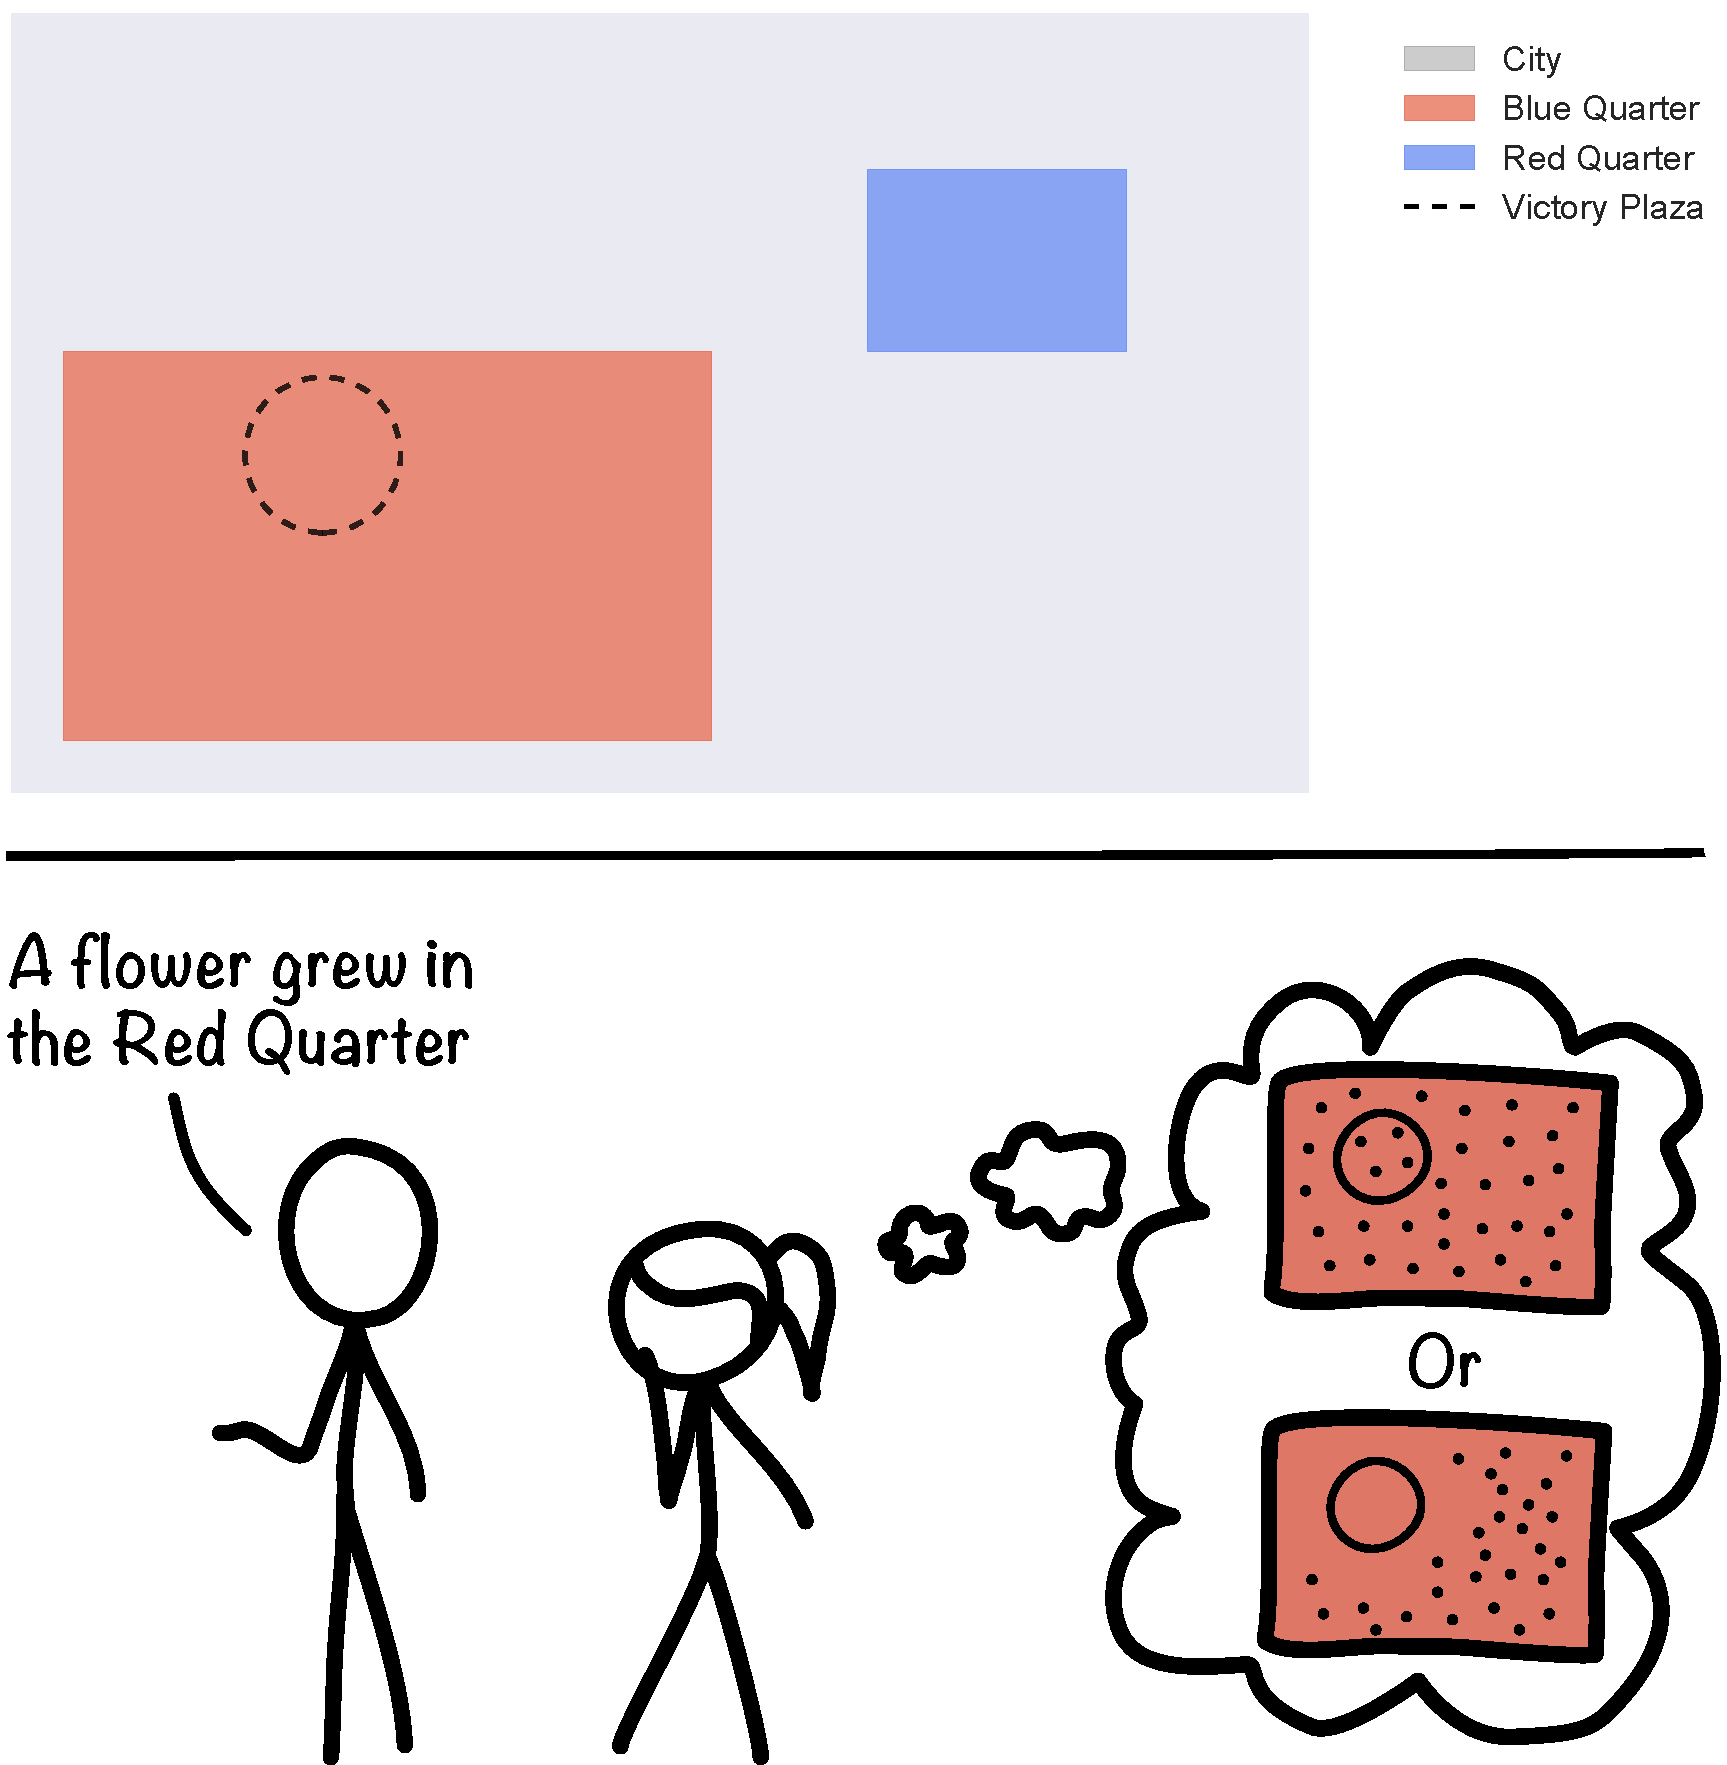
\includegraphics[width=.5\textwidth]{figures/illustration2.pdf}
\caption{Illustration of a simple spatial situation.}
\label{illustration}
\end{figure}

%In this study, we explore the relation between pragmatics and spatial language using probabilistic programs~\cite{}. MAYBE NOAH CAN SAY SOMETHING HERE? 

% To preview our results ... MAYBE TOMER CAN FILL IN THE EXCITING RESULTS PREVIEW HERE? \ndg{or we could just move on to the meat....}

\section{Modeling spatial implicature}\label{mod}

We model spatial language understanding within the Rational Speech Acts (RSA) framework of \citeA{frankgoodman2012,ndg+ast:topics2013}.
This has previously been applied to domains such as object properties with terms such as quantifiers (e.g.~``some of the apples are red'' implying that a subset of the apples are red).
We adopt this framework to spatial language by taking locations as the domain of interest and building a lexicon for describing spatial relations. 
The RSA framework specifies a pragmatic listener reasoning about the intention of an informative speaker, who in turn reasons about a literal listener; the literal listener updates her beliefs by conditioning on the truth of the utterance.
Altogether, writing the position of interest (e.g.~of the Golden Lily) as $s$ and the utterance (e.g.``in the red quarter'') as $u$:
\begin{eqnarray}
P_{L_1}(s|u)&\propto&P_{S_1}(u | s) P(s) \label{eqn:L1}\\
P_{S_1}(u|s)&\propto&\sum_{s' \text{ s.t. } |s-s'|<\epsilon} P_{L_0}(s'|u) P(u)\label{eqn:S1}\\
P_{L_0}(s|u)&\propto& \delta_{\denote{u}(s)} P(s)\label{eqn:L0}
\end{eqnarray}
Beginning with the simplest listener model, $L_0$, Equation \ref{eqn:L0} specifies a listener who interprets the utterance via its truth-functional denotation, $\denote{u}$ described in more detail below, and simply restricts the prior distribution over locations to those where this denotation is true.
The speaker, $S_1$, in Equation \ref{eqn:S1} aims for the literal listener to guess the correct location, balanced against the prior probability (i.e.~cost) of the utterance. \ndg{do we use cost here? if not remove from eqns.}
However, because it is vanishingly unlikely for $L_0$ to guess exactly the right location, our speaker only cares if the location is within a small distance $\epsilon$; this corresponds to an \emph{approximate question under discussion} as used by \citeA{kao2014}.
Finally, the pragmatic listener, $L_1$, in Equation \ref{eqn:L1} updates her beliefs in accord with Bayes' rule, under the assumption that the $S_1$ speaker would have chosen the utterance she heard.





%spatial implicature using the rational speaker-listener model applied previously to domains such as scalar implicature and social reasoning \cite{ndg+ast:topics2013,ast+ndg:cogsys2013}. We consider a speaker and listener as in the sketch shown in Figure (**). Both speaker and listener have access to a shared lexicon that contains a mapping from possible utterances to predicates that return Boolean values over states of the world. For example, in our specific lexicon the utterance ``in Red Quarter'' maps to a predicate that takes in a location  and returns the value $True$ if that location falls within the boundaries of the Red Quarter rectangle, and $False$ otherwise. We expand on the lexicon details further down. 
%
%The listener attempts to infer the true state of where an event occurred in the world ($s$), by considering the utterance they heard from the speaker ($u$), and the listener's knowledge of the world and the speaker. We consider two possible listeners. The first is a \textit{literal} listener ($L_0$) who understands an utterance by strictly referring to its meaning in a lexicon, modulated by the prior probability of a state occurring:
%
%\begin{equation}
%P_{L_0}(s|u)\propto P(s|u(s)=True)P(u),
%\end{equation}
%
%A speaker faced with such a literal listener ($S_0$) will choose an utterance that will maximize the probability of the listener inferring the correct state $s$. In continuous spatial distributions an exact equality between the observed state $s$ and the listener's inferred state $s'$ cannot be expected, and it is only required that an approximate equality condition holds $s\approx s'$. In this paper we use $|s-s'|<\epsilon$, though other approximate equality conditions are possible. The speaker is then:
%
%(*** Not sure about the exact equation to put down here ***)
%\begin{equation}
%P_{S_0}(u|s)\propto ***
%\end{equation}
%
%The second possible listener is a \textit{pragmatic} listener ($L_1$), who takes into account the speaker's reasoning when choosing an utterance:
%
%\begin{equation}
%P_{L_1}(s|u)\propto P_{S_0}(u|s)P(s)
%\end{equation}
%
%Such recursive, probabilistic reasoning can be captured as a probabilistic program. We implemented the model in the Church language (cite, website?) along the following lines: \\
%
%\texttt{({\color{blue}{define}} (speaker state)}\\
%\texttt{\tab ({\color{blue}{rejection-query}}}\\
%\texttt{\tab  ({\color{blue}{define}} utterance (sample utterance-prior))}\\
%\texttt{\tab   \color{BurntOrange};; Return utterance...}\\
%\texttt{\tab   utterance}\\
%\texttt{\tab   \color{BurntOrange};; Conditioned on...}\\
%\texttt{\tab  (about-equal state (listener utterance 0))))}\\
%\texttt{}\\
%\texttt{({\color{blue}{define}} (listener utterance depth)}\\
%\texttt{\tab ({\color{blue}{rejection-query}}}\\
%\texttt{\tab  (define state (sample state-prior))}\\
%\texttt{\tab   \color{BurntOrange};; Return state...}\\
%\texttt{\tab  state}\\
%\texttt{\tab   \color{BurntOrange};; Conditioned on...}\\
%\texttt{\tab  ({\color{blue}{if}} (= depth 0)}\\
%\texttt{\tab \tab \tab  (utterance state)}\\
%\texttt{\tab \tab \tab  (equal? utterance (speaker state))))}\\
%
%Listeners of depth 0 and 1 are \textit{literal} listener $L_0$ and \textit{pragmatic} listener $L_1$ as defined above. While higher combinations of listener and speaker depths are useful in games of social coordination (CITE), in many tasks the \textit{pragmatic} listener model is sufficient, and here we are interesting is seeing how well it models people's behavior in a spatial task above that of a \textit{literal} listener. 

%\subsubsection{Lexicon} 


The denotation of an utterance $u$ is a function from position to Boolean: $\denote{u}(s)\in \text{Bool}$.
We will assume that the spatial language relevant to our scenarios depends on a context set of regions in $\mathbb{R}^2$.
(As in Figure \ref{illustration}: The City, The Red Quarter, The Blue Quarter, The Victory Plaza.)\footnote{Both the denotation and Equations \ref{eqn:L0}-\ref{eqn:L1} depend on the context of named regions. We leave this dependence implicit to avoid clutter.}
%The utterances are implemented as boolean functions that take in a state of the world (the x,y pair where an event occurred) and return $True$ or $False$. 
We considered three types of spatial utterances, each of which combines a preposition with a region name: 
\begin{itemize}
\item ``In'' utterances (e.g. ``In the Red Quarter'') are true within the region: $\denote{\text{``in R''}}(s) := s\in R$.
\item ``Near-edge'' utterances (e.g. ``Near the edge of the Red Quarter'') are true within distance $d$ of a region boundary: $\denote{\text{``near edge R''}}(s) := \mu(s,\beta(R))<d$. (Where $\mu$ measure distance to a set, and $\beta$ returns the boundary of a region.)
\item ``Near'' utterances (e.g. ``Near the Red Quarter'') are true near the edge but not inside: $\denote{\text{``near R''}}(s) := 
\denote{\text{``near edge R''}}(s) \wedge \neg \denote{\text{``in R''}}(s)$.
\end{itemize}
People no doubt have access to many more spatial utterances, and their combinations, but we restrict ourselves to this set for simplicity. 


% return $True$ if the event falls within the boundaries of a region and $False$ otherwise. ``Near-edge'' utterances (e.g. ``Near the edge of the Red Quarter'') return $True$ if the event is within a distance $d$ of the boundaries of a region and $False$ otherwise. ``Near'' utterances (e.g. ``Near the Red Quarter'') return $True$ if the event is near the edge of a region but not in it, as defined by the ``In'' and ``Near-edge'' utterances. 



%\subsubsection{Parameter choice} 

The model as stated leaves open the question of what distance counts as ``Near'' or ``Near the edge'' in the shared lexicon (what $d$ to use), as well as what counts as ``approximately equal'' between the true state and the inferred state (what $\epsilon$ to use). We set $\epsilon$ to 10 units (pixels), based on initial exploration. 
Because the intuitive flexibility of ``Near'' seems to depend on the item and context (``near your coffee mug'' is not the same as ``near your coffee house''), we allow the literal listener to establish the most useful $d$ for each utterance.
We extend Equation \ref{eqn:L0} to include uncertainty about the tolerances for each ``near'' utterance:
\begin{equation}
P_{L_0}(s|u)\propto \sum_{\vec{d}} \delta_{\denote{u}_{\vec{d}}(s)} P(s) P(\vec{d})\label{eqn:L0tol},
\end{equation}
where $\vec{d}$ is a real number, the tolerance, for each utterance. We assume $P(\vec{d})$ is uniform over \ndg{some range}.

We implement this model in the probabilistic programming language Church \cite{goodman2008}. A full implementation can be found at \url{http://forestdb.org/models/spatialImplicature.html}. We used this implementation to generate predictions for each spatial configuration (``city'') used in the experiment below, and for each utterance.


\begin{figure*}[!t]
\center
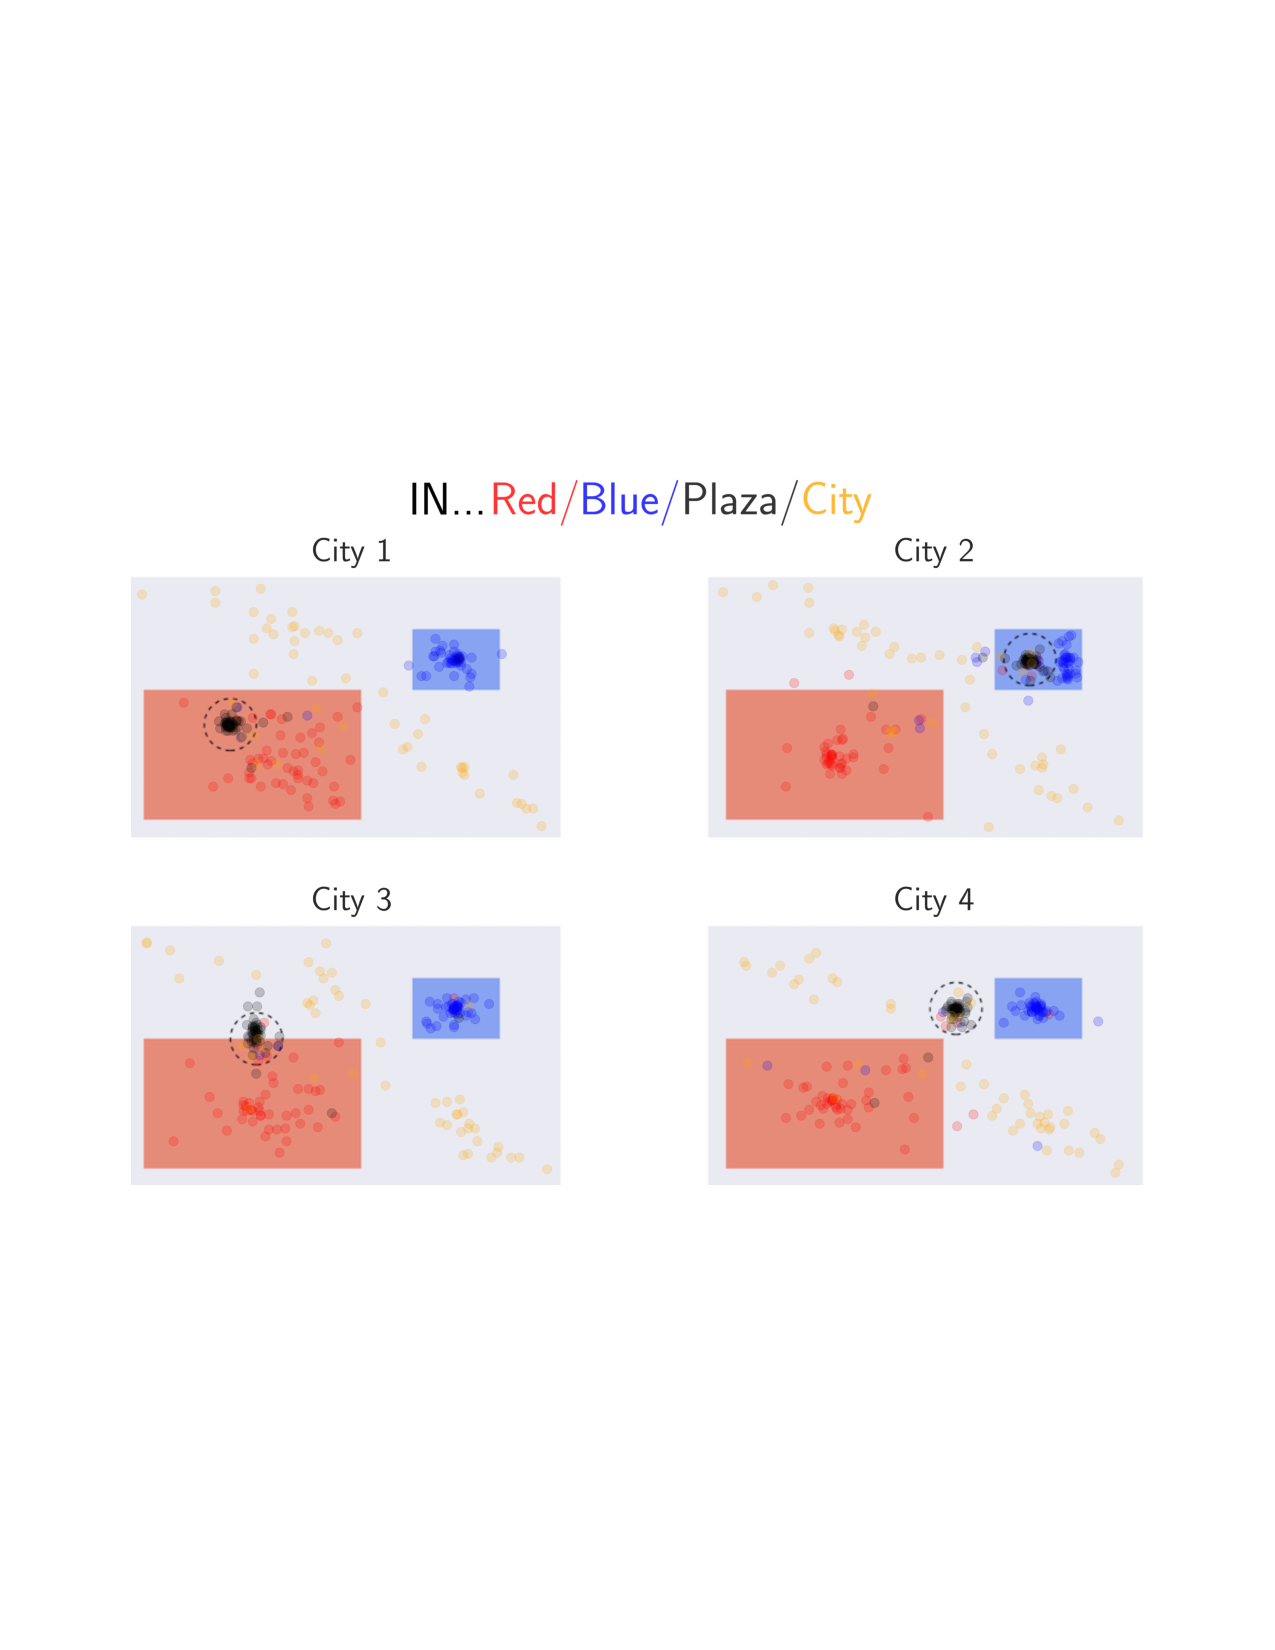
\includegraphics[width=.82\textwidth]{figures/In.pdf}
\caption{Results across `In' utterances. Dots are guesses of where a Gold Lily grew, color coded by region `In' refers to.}
\label{fig:In}
\end{figure*}

\begin{figure*}[!]
\center
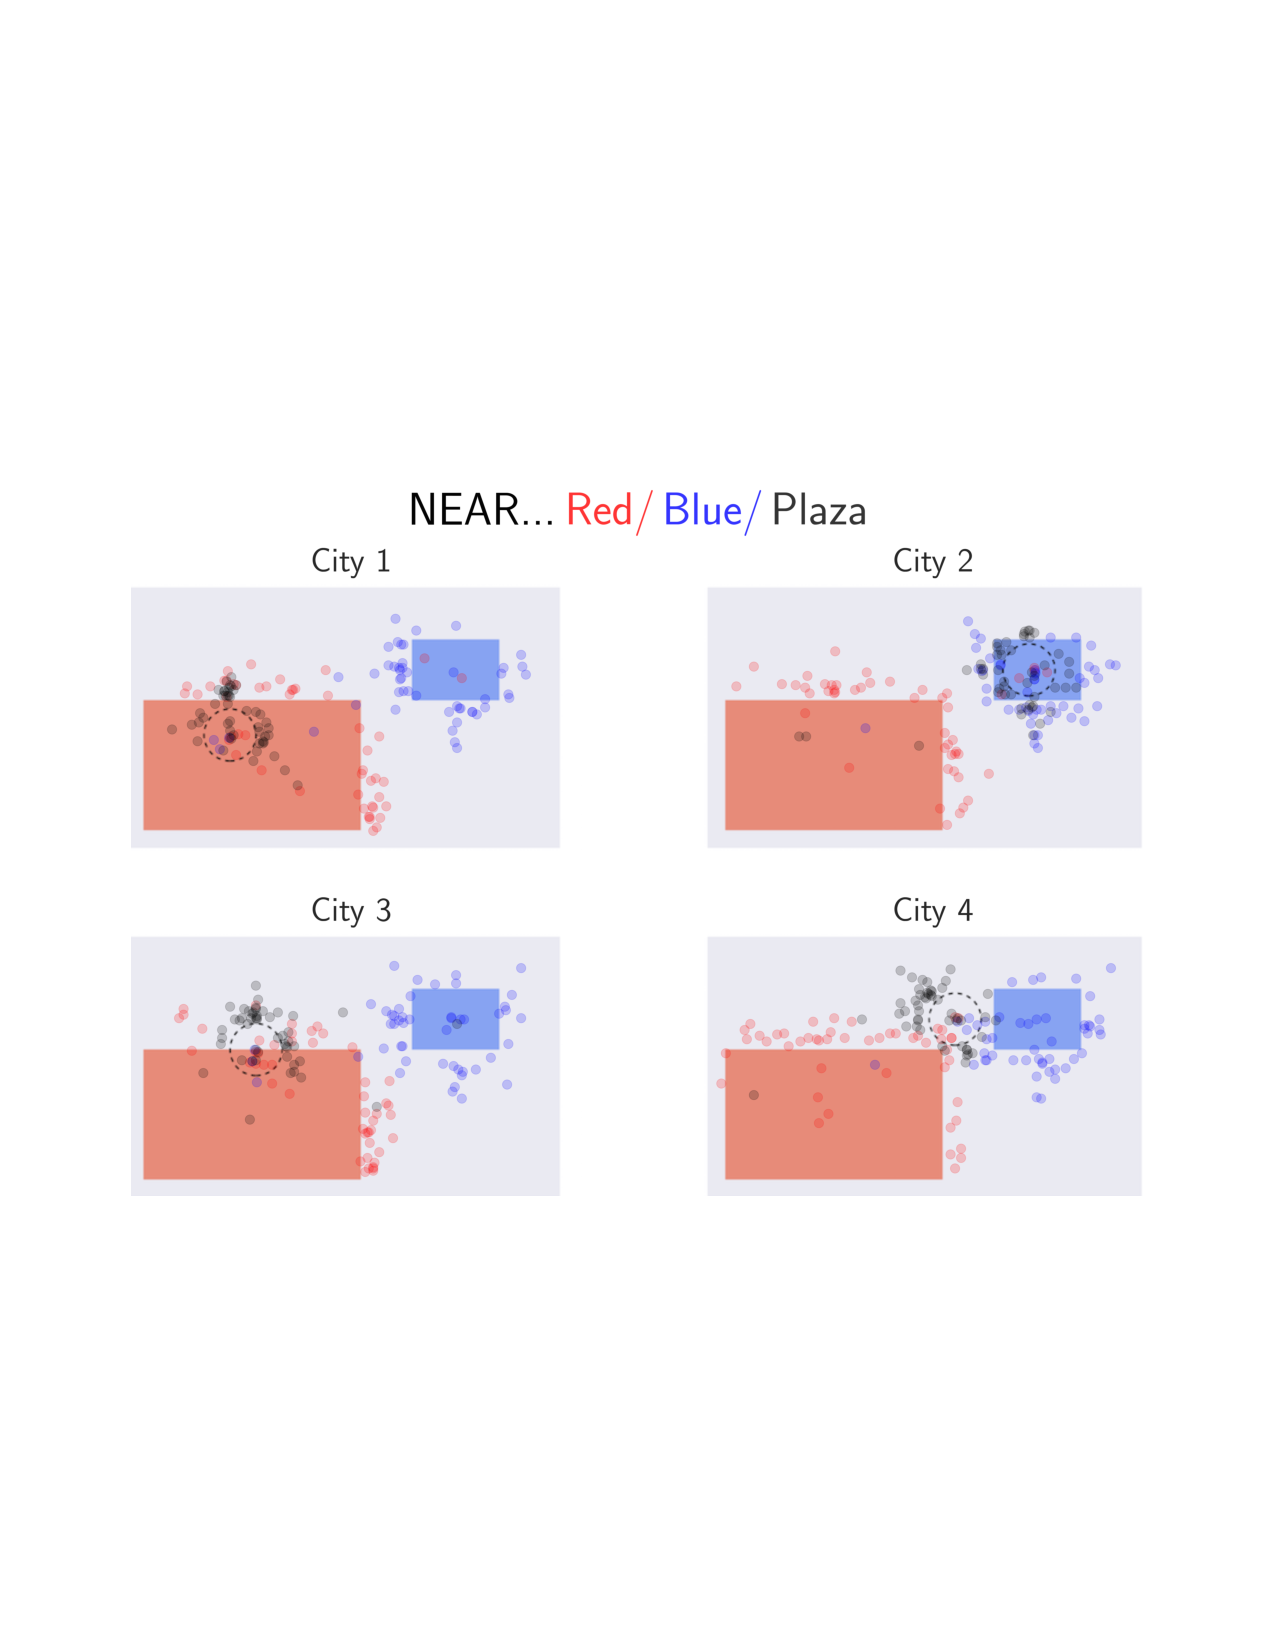
\includegraphics[width=.82\textwidth]{figures/Near.pdf}
\caption{Results across `Near' utterances.}
\label{fig:Near}
\end{figure*}

\section{Experiment}\label{sec:exps}

We examined people's spatial inferences and the predictions of our model regarding the spatial terms `in' and `near', by putting participants in the role of a listener and asking them to guess where an event happened on a map in response to an utterance of a speaker who had access to the location of the event. 

\subsection{Participants, materials and methods}

Participants ($N=49$, 13 female, median age 29) were recruited through Amazon's Mechanical Turk service. 

We constructed 4 simple city maps (see Fig. XX), each containing 2 ``Quarters'' of different size and color, and a circle marked as ``Victory Plaza''. The location of Victory Plaza varied among the 4 cities, while the location of the Quarters remained the same. To broadly control for effects of color and position, we created another set of 4 maps by flipping the original maps along the vertical and horizontal axis, and changing the color of the quarters, making 8 maps in total. Participants were randomly assigned to one of the two map groups. 

\begin{figure*}[!t]
\center
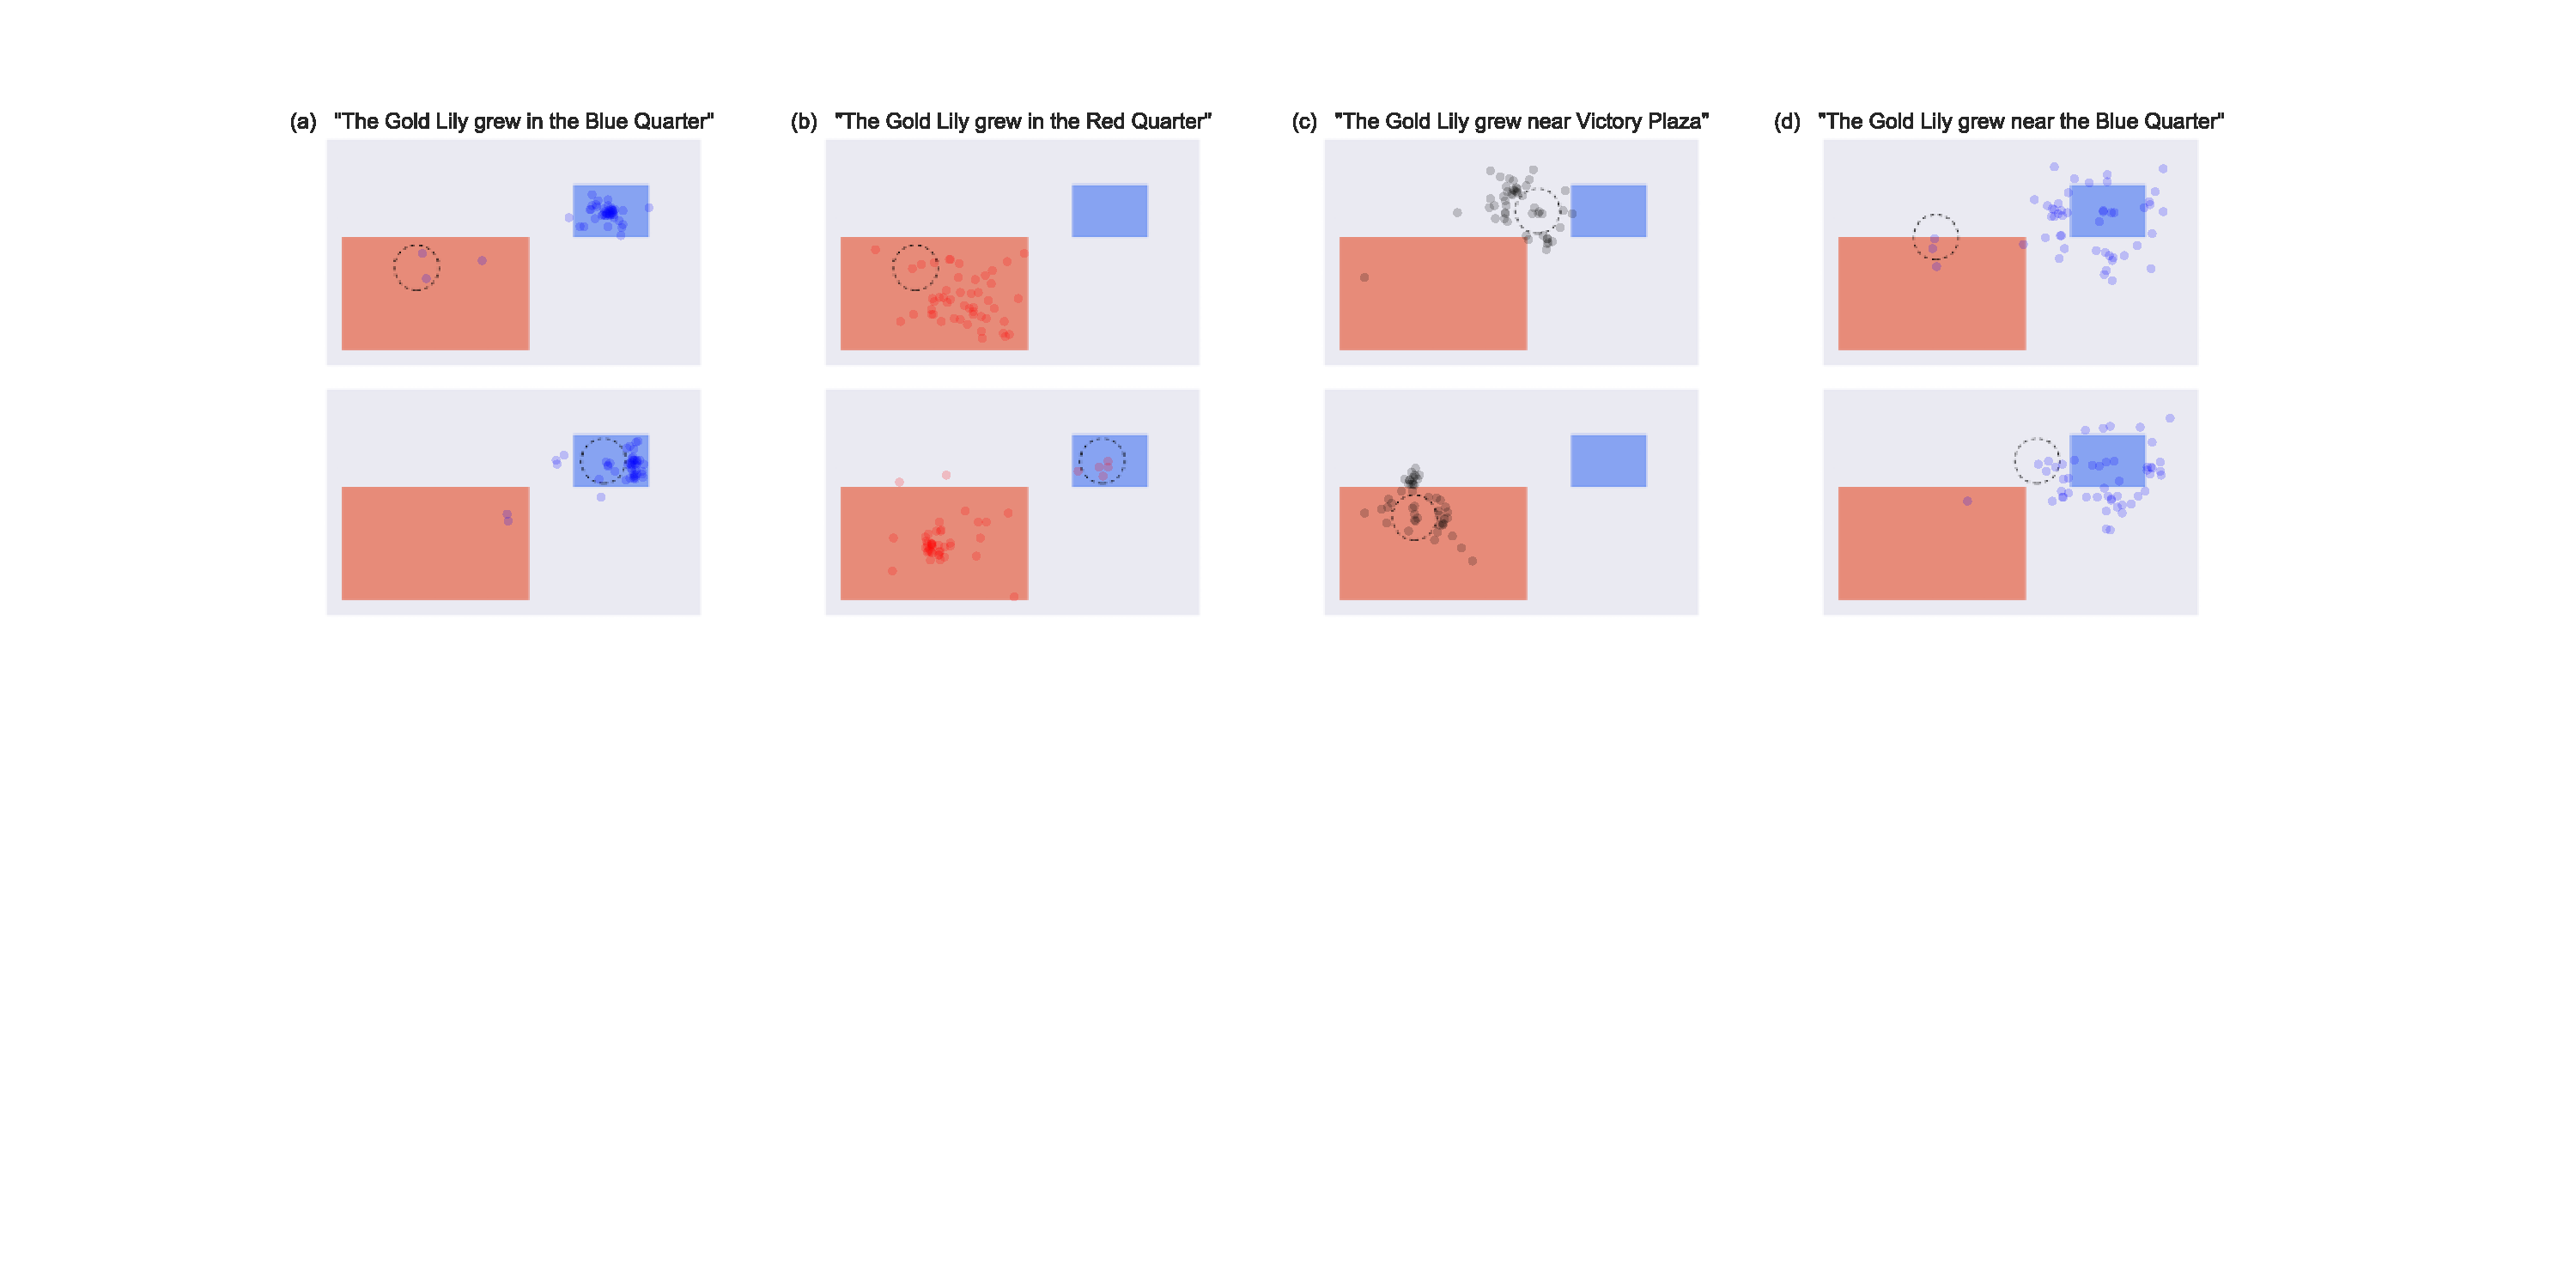
\includegraphics[width=\textwidth]{figures/results1.pdf}
\caption{zoom in on results}
\label{fig:zoomIn}
\end{figure*}

Participants were shown an example map including a legend (as in Figure ***), and were informed that throughout the experiment they would see similar maps. Participants were told that anywhere in the city they're shown, a special flower called a `Gold Lily' can grow, and that their task is to find the Gold Lilies. 

Participants were further told that in their task a person will tell them where a Gold Lily grew, and that this person can say the Gold Lily grew \textit{in} a location or \textit{near} a location. This person was also said to be reasonable, and honest. As an example, a participant might read the sentence `A person tells you: A Gold Lily grew in the Red Quarter'. Participants made their guess by clicking directly on the maps they were shown.

For each of the 4 maps in their group, participants were prompted with a sentence made of $word \times location$ combinations, where $word \in [In,\ Near]$ and $location \in [Red\ Quarter,\ Blue\ Quarter,\ Victory\ Plaza,\ City]$. We chose not to include the combination ``Near the City'', as this area was not in the scope of the image and likely to create confusion. In total, each participant was prompted with 28 different sentences, shown in random order. Each map had a legend clearly displayed to its right. 

\subsection{Qualitative Results} 

Figure \ref{fig:In} shows participants' guesses for ``in'' sentences and Figure \ref{fig:Near} shows guesses for ``near,'' collapsing across the rotated-and-inverted-color cities and color-coded by the region referred to. For example, in the top-left of Figure \ref{fig:In}, the blue dots correspond to all participant guesses for where the Gold Lily grew in City 1 when prompted with ``In the Blue Quarter''. 

To explore qualitative effects, we will focus on the cases highlighted in Figure \ref{fig:zoomIn}. The reader is encouraged to examine the remaining twenty cases, which show similar effects. 

%Any combination of word, location and city out of the 28 possibilities is informative, but space does not allow out. Instead, we focus on several general findings, making reference to particular examples in Figure \ref{fig:zoomIn}, and the reader is encouraged to consider other combinations for themselves.

\subsubsection{`In X' implies `In X but not in Y'} As shown for example in Figure \ref{fig:zoomIn}(a): When people hear `In Blue' in City 2 (bottom) they infer `In Blue, but not in the Plaza'. Both the top and bottom of (a) show participant guesses for the lily location when told it grew in the Blue Quarter. In the top figure (Blue Quarter without Plaza) people place most of their guesses in the center of the Quarter (a tic-tac-toe-like division of the Quarter shows that the grid center, accounting for 11\% of the area, captures 59\% of the guesses). In the bottom figure (Blue Quarter with Plaza), people avoid the same center (the grid center captures 8\% of the guesses) while shifting to the right of the Plaza. Such a pattern of results holds for the other regions as well, as shown in Figure \ref{fig:In}. 

\subsubsection{Edge avoidance} When there is no direct intersection between regions (except with the City, which all regions intersect with), people do not guess uniformly in the region, but rather favor the center. For example, in Figure \ref{fig:zoomIn}(b), bottom: When people hear `In Red' they place most of their guesses in the center of the region. A grid-analysis shows the red-grid center accounts for 65\% of the guesses, as opposed to the 11\% expected by chance. Using 10,000 bootstrapped simulations of 49 subjects drawn from a uniform distribution on the Red Quarter shows that in \textit{none} of them does the center account for more than ~30\% of the responses. 

\subsubsection{`Near' is non uniform on edges} As shown in Figure \ref{fig:zoomIn}(c) and (d), when told `Near Plaza' or `Near Blue', people do not place a uniform probability on edges of regions, and where they guess depend on the context of other regions.
In (c), people place most of their guesses to the top-left of the Plaza (top) or in the top and right of the Plaza (bottom). In (d), people place most of their guesses to the left and bottom of the Blue Quarter (top) or the bottom of the Blue Quarter (bottom). 
\ndg{some simple stat showing that guesses are not uniform and depend on context? eg counts in the four quadrants wrt the plaza?}

\ndg{it would be nice to say something qualitative about the distance from the boundary for ``near''. can we show that it differs by object/context?}

This qualitative pattern of results make it clear that context affects participants' interpretations of spatial language, as expected under a pragmatic account.
%While showing some examples of spatial implicature, this pattern of results is explicitly qualitative. 
In the next section, we turn to a quantitative analysis, comparing results with the different listener models described above. 

\section{Comparison to Model(s)}

\begin{figure*}[!t]
\center
\includegraphics[width=\textwidth]{figures/Figure4.pdf}
\caption{Example comparisons between people and the two listener models. Colored patches indicate probability distributions inferred from people's responses and model samples. Numbers to the right of each listener subplot indicate the $KL$ distance between the distributions of people and the model samples, lower is better.}
\label{fig:modelExamples}
\end{figure*}

In order to quantitatively compare people to the literal listener and pragmatic listener models ($L_0$ and $L_1$), we converted their responses into smooth two-dimensional distributions. We used non-parametric, multivariate kernel density estimation to infer these distributions \ndg{cite?}. The same estimation procedure was applied to samples drawn from the probabilistic programs that represent the $L_0$ and $L_1$ models. 

Example comparisons are shown in Figure \ref{fig:modelExamples}. When hearing `In Red' in City 1 (left-most column) The literal listener $L_0$ places a uniform posterior distribution on the Red Quarter, while $L_1$ and people avoid Victory Plaza and lean to the right of the Red Quarter. This correspondence can be measured in terms of the Kullback–-Leibler ($KL$) distance between the distributions. In this particular example, $KL(\text{people} | L_0) = 0.43$, while $KL(\text{people} | L_1) = 0.25$. 
The pragmatic listener $L_1$ is closer to people than the literal listener for 26 of the 28 (93\%) possible comparisons. Figure \ref{fig:KL} shows the distribution of the distances for both listener models. 

As Figure \ref{fig:modelExamples} shows, the $L_1$ model captures many of the interesting implicature-like interpretations shown by people.
%examples of correspondence between people's implicature inferences and $L_1$. 
Indeed, the $L_1$ listener shows the same general qualitative patterns discussed in the previous section. A full comparison figure is would exceed the space limits of this paper, but can be found here: (*LINK*).

\begin{figure}[!t]
\center
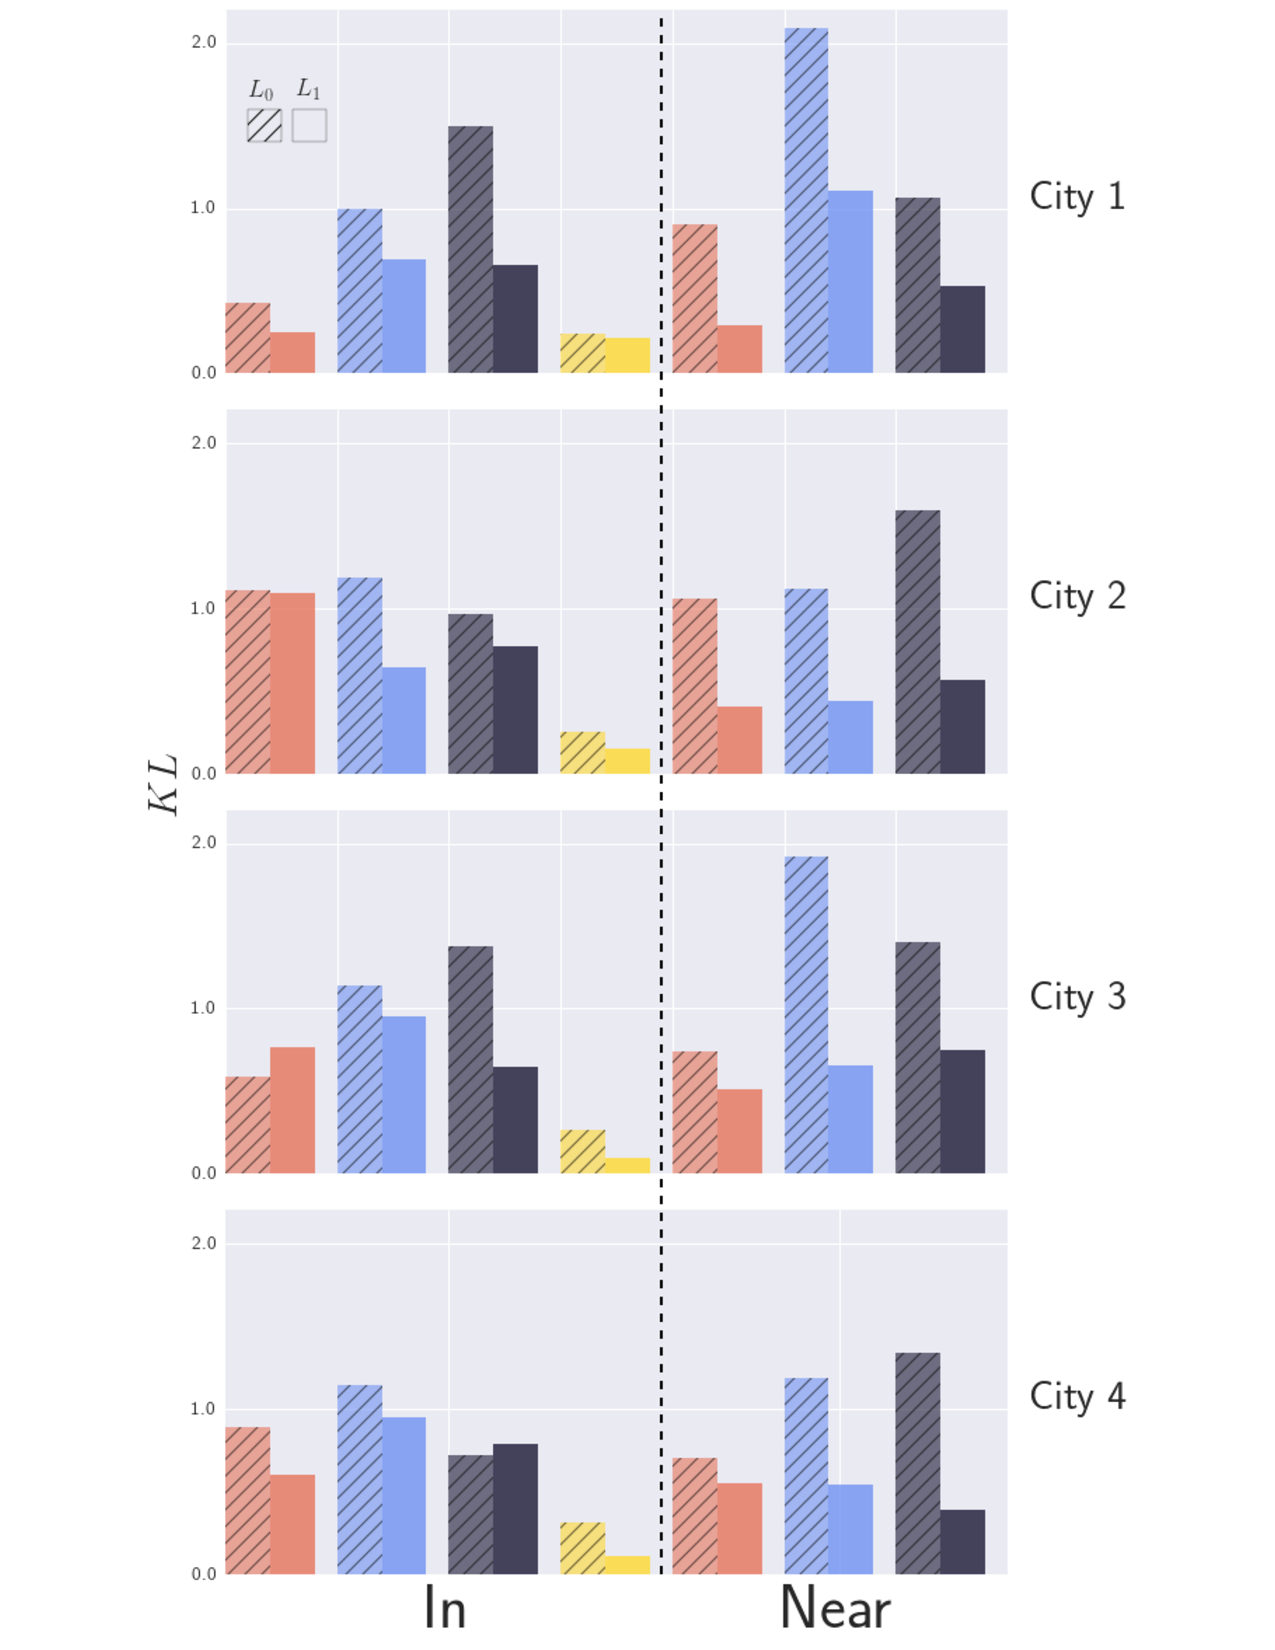
\includegraphics[width=0.45\textwidth]{figures/KL.pdf}
\caption{KL distances between distributions inferred from people and the two listener models, organized by question and city. Hatched bars are the literal listener $L_0$ and plain bars are the pragmatic listener $L_1$. The color of the bar codes the question as before.}
\label{fig:KL}
\end{figure}


\ndg{i wonder what it would look like to make a model-data scatter plot by binning counts on a grid?}

These results suggest that the pragmatic listener model is able to account for the quantitative pattern of pragmatic spatial inferences of people, within our domain.  

\section{Discussion}

\ndg{discuss some stuff....}


%%%%%%%%

\bibliographystyle{apacite}
\setlength{\bibleftmargin}{.125in}
\setlength{\bibindent}{-\bibleftmargin}
\bibliography{cogscibib}
\end{document}
